\newpage
\subsection{File System}

\subsubsection{Size of file cache}

// NOTE
Note that this may be very sensitive to other load on the machine. Report results as a graph whose x-axis is the size of the file being accessed and the y-axis is the average read I/O time. Do not use a system call or utility program to determine this metric except to sanity check.
// NOTE
% Data and cmd line to change unit
%
%NoKriK-20:~ nokrik$ sed 's/MB//' /tmp/cacheperf  | awk '{ print $0, "Avg speed
%=", (1 / ($8 / 3300000000.)) * $6, "MB/s" } '
%
%Average cycles for file of 128 = 350521462.800000 Avg speed = 1205.06 MB/s
%Average cycles for file of 256 = 714140116.200000 Avg speed = 1182.96 MB/s
%Average cycles for file of 384 = 1058802582.900000 Avg speed = 1196.82 MB/s
%Average cycles for file of 512 = 1378372357.800000 Avg speed = 1225.79 MB/s
%Average cycles for file of 640 = 1685485896.000000 Avg speed = 1253.05 MB/s
%Average cycles for file of 768 = 2035878978.000000 Avg speed = 1244.87 MB/s
%Average cycles for file of 896 = 2346212095.200000 Avg speed = 1260.24 MB/s
%Average cycles for file of 1024 = 2689287792.900000 Avg speed = 1256.54 MB/s
%Average cycles for file of 1152 = 3042130221.900000 Avg speed = 1249.65 MB/s
%Average cycles for file of 1280 = 3422302482.100000 Avg speed = 1234.26 MB/s
%Average cycles for file of 1408 = 54968266452.099998 Avg speed = 84.5288 MB/s
%Average cycles for file of 1536 = 76498366019.600006 Avg speed = 66.2602 MB/s
%Average cycles for file of 1664 = 63298490339.900002 Avg speed = 86.7509 MB/s
%Average cycles for file of 1792 = 76528285416.000000 Avg speed = 77.2734 MB/s
%Average cycles for file of 1920 = 77574515912.000000 Avg speed = 81.6763 MB/s
%Average cycles for file of 2048 = 81218869075.899994 Avg speed = 83.2122 MB/s
%Average cycles for file of 2176 = 89535122151.000000 Avg speed = 80.2009 MB/s
%Average cycles for file of 2304 = 104532359347.199997 Avg speed = 72.7354 MB/s
%Average cycles for file of 2432 = 102806365027.600006 Avg speed = 78.0652 MB/s



\paragraph{Methodology}
We created a file of 128MB and we expanded it up to 2432MB.
Each 128MB written, we read the file 10 times and averaged the result.
We use the low level routine \emph{read} to avoid the caching of the stdio
functions.
We converted the data from cycles to MB/s and then ploted them.

\paragraph{Predictions}
Our solaris 11 system uses the ZFS filesystem as root filesystem.
ZFS is using an Adaptive Replacement Cache (ARC) which is growing dynamicly
depending on the usage of the filesystem and on the main memory usage.
We except the cache to be a bit less than our idle free memory, so less than
1345MB.
The performance will degrade from the 1408MB file and reach a speed near the
speed of the hardware disks.

The memory need to be copied from kernel space to user space by chunk of the
user land buffer size.
The memory operations cost can be estimated by averaging the read and the write
bandwidth and dividing the result by 2.
With this method, we can estimate the bandwidth to 4GB/s.

As seen before, a minimum system call cost about 800 cycles.
\emph{read} is more complexe and should take around 1000 cycles to proceed.
Our userland buffer is 2KB which implies a cost of 79ms per GB read due to the
syscall overhead.
Accounting with this software overhead, the predicted bandwidth falls to 3.59GB/s.

\paragraph{Results}
\begin{table}[h]
\begin{center}
\begin{tabular}{| l | l | l | l | l |}
\hline
File size & Hardware bandwidth & Software cost & Prediction & Measured \\
128MB  & 4GB/s   & 79ms/GB & 3.59GB/s & 1205.06 MB/s \\ \hline
256MB  & 4GB/s   & 79ms/GB & 3.59GB/s & 1182.96 MB/s \\ \hline
384MB  & 4GB/s   & 79ms/GB & 3.59GB/s & 1196.82 MB/s \\ \hline
512MB  & 4GB/s   & 79ms/GB & 3.59GB/s & 1225.79 MB/s \\ \hline
640MB  & 4GB/s   & 79ms/GB & 3.59GB/s & 1253.05 MB/s \\ \hline
768MB  & 4GB/s   & 79ms/GB & 3.59GB/s & 1244.87 MB/s \\ \hline
896MB  & 4GB/s   & 79ms/GB & 3.59GB/s & 1260.24 MB/s \\ \hline
1024MB & 4GB/s   & 79ms/GB & 3.59GB/s & 1256.54 MB/s \\ \hline
1152MB & 4GB/s   & 79ms/GB & 3.59GB/s & 1249.65 MB/s \\ \hline
1280MB & 4GB/s   & 79ms/GB & 3.59GB/s & 1234.26 MB/s \\ \hline
1408MB & 100MB/s & ?       & ?        & 84.5288 MB/s \\ \hline
1536MB & 100MB/s & ?       & ?        & 66.2602 MB/s \\ \hline
1664MB & 100MB/s & ?       & ?        & 86.7509 MB/s \\ \hline
1792MB & 100MB/s & ?       & ?        & 77.2734 MB/s \\ \hline
1920MB & 100MB/s & ?       & ?        & 81.6763 MB/s \\ \hline
2048MB & 100MB/s & ?       & ?        & 83.2122 MB/s \\ \hline
2176MB & 100MB/s & ?       & ?        & 80.2009 MB/s \\ \hline
2304MB & 100MB/s & ?       & ?        & 72.7354 MB/s \\ \hline
2432MB & 100MB/s & ?       & ?        & 78.0652 MB/s \\ \hline
\end{tabular}
\end{center}
\caption{Size of file cache\label{tab:file-cache}}
\end{table}

\begin{figure}[h]
\begin{center}
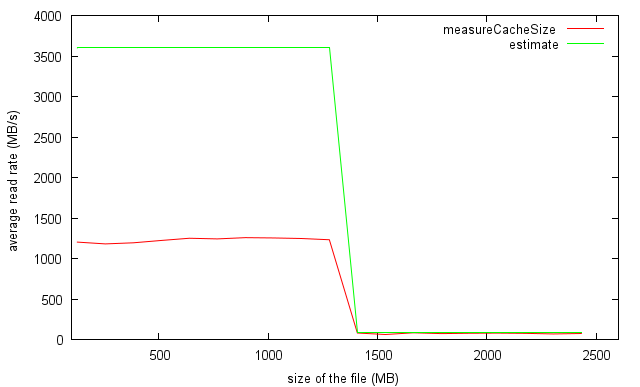
\includegraphics[scale=0.8]{fileCacheImage}
\end{center}
\caption {File cache\label{fig:file-cache}}

\end{figure}

According to the result shown in table \ref{tab:file-cache} and figure \ref{fig:file-cache}, we can see that the cache
is between 1280MB and 1408MB.
Our prediction were correct and the file size cache grew until it would have
needed to swap out other applications.
The bandwidth is much lower than excepted. 

\paragraph{Success of Methodology}



\subsubsection{File read time}

//NOTE
Report for both sequential and random access as a function of file size. Discuss the sense in which your "sequential" access might not be sequential. Ensure that you are not measuring cached data (e.g., use the raw device interface). Report as a graph with a log/log plot with the x-axis the size of the file and y-axis the average per-block time.
//NOTE

\paragraph{Methodology}
Solaris has a library function called \emph{directio} which is supposed to
enable filesystem cache bypassing.
The function is not supported with ZFS so we were forced to reduce the
filesystem cache size manually with the \emph{mdb} command\cite{zfs-evil-tuning}.
We couldn't reduce the cache lower than 64MB as ZFS doesn't allow
it\cite{zfs-arc-max}.

We then created a file of 2MB and read it 10 times sequentially and read the
size of the file randomly 10 times.
For the random read, we used the urandom function to generate an offset in the
file and we used the \emph{lseek} system call to move to the position in the file.

The read are read of 128KB as ZFS is dynamicly adjusting the block size up to
128KB and our files are big.
We also took care of reading on 128KB aligned values.

\paragraph{Predictions}
The sequential access are usually not really sequential depending of the
fragmentation of the file system.
We except to reach 90\% of the bandwidth of the disk on sequential reads
and a low disk latency.
The file are newly written files and the partition is not full so the filesystem
should not be much fragmented.

For the random file read time, we except a higher latency per block access.
The random access patern will directly show the latency of the disk.
The average access time of the disk is 18ms.
The locality should still be better than a total random read so the average
latency should be lower than this.
As the average access time is about 18ms, the disk should be able to handle
about 55 random IOPS.
In our test program, each read is 2048 bits, the worst result should be about 110 kB/s.

\paragraph{Results}
\begin{table}[h]
\begin{center}
\begin{tabular}{| l | l | l | l | l |}
\hline
Operation & Hardware cost & Software cost & Prediction & Measured \\
\hline
\end{tabular}
\end{center}
\caption{File read time\label{tab:file-read-time}}
\end{table}

\begin{figure}[h]
\begin{center}
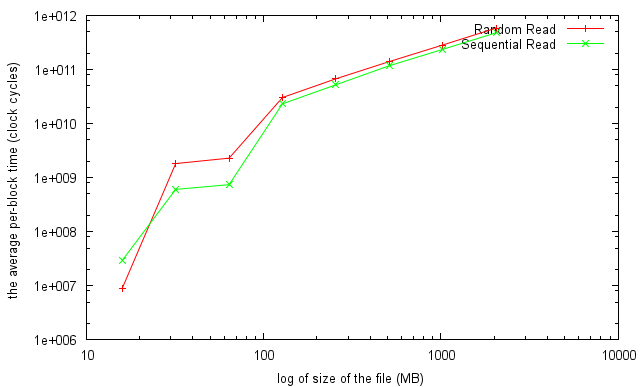
\includegraphics[scale=0.8]{fileAccessImage}
\end{center}
\caption {File cache\label{fig:file-access}}

\end{figure}


According to the result shown in table \ref{tab:file-read-time} and figure \ref{fig:file-access}, we


\paragraph{Success of Methodology}
We wern't able to measure the performance for small files as ZFS doesn't support
direct i/o and we couldn't reduce the cache so that the small files doesn't fit
into the cache.





\subsubsection{Remote file read time}
//NOTE
Repeat the previous experiment for a remote file system. What is the "network penalty" of accessing files over the network?
//NOTE

\paragraph{Methodology}

\paragraph{Predictions}
\paragraph{Results}

\begin{table}[h]
\begin{center}
\begin{tabular}{| l | l | l | l | l |}
\hline
Operation & Hardware cost & Software cost & Prediction & Measured \\
\hline
\end{tabular}
\end{center}
\caption{Remote file read time\label{tab:remote-file-access}}
\end{table}

According to the result shown in \ref{tab:remote-file-access}, we
\paragraph{Success of Methodology}




\subsubsection{Contention}
//NOTE
Report the average time to read one file system block of data as a function of the number of processes simultaneously performing the same operation on different files on the same disk (and not in the file buffer cache).
//NOTE

\paragraph{Methodology}

\paragraph{Predictions}
\paragraph{Results}
\begin{table}
\begin{center}
\begin{tabular}{| l | l | l | l | l |}
\hline
Operation & Hardware cost & Software cost & Prediction & Measured \\
\hline
\end{tabular}
\end{center}
\caption{Contention\label{tab:contention}}
\end{table}

According to the result shown in \ref{tab:contention}, we

\paragraph{Success of Methodology}
